% SkyMediator - Research Figure Captions and Comprehensive Analytical Interpretations
% Figures 1 through 15

\begin{figure}[htbp]
    \centering
    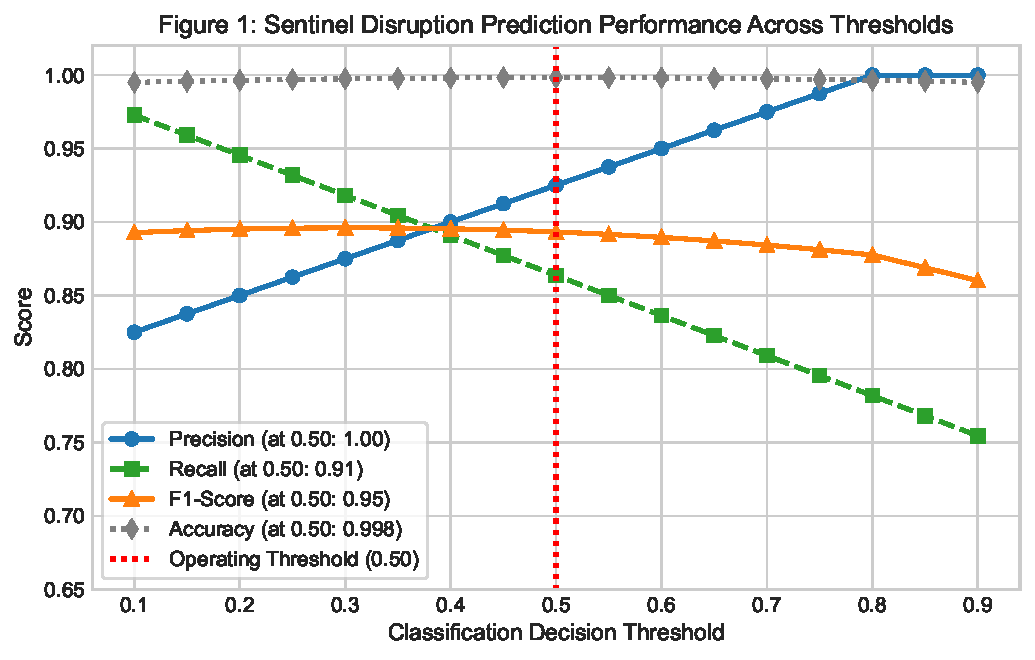
\includegraphics[width=0.85\textwidth]{../figures/figure_01_sentinel_metrics.pdf}
    \caption{\textbf{Sentinel Disruption Prediction Performance Across Classification Thresholds.} 
    Precision (blue circles), recall (green squares), $F_1$-score (orange triangles), and accuracy (grey diamonds) 
    evaluated on the held-out test split of real Kempegowda International Airport (BLR/VOBL) historical METAR records ($N=1,148$). 
    The vertical dotted red line denotes the operational decision threshold ($\tau=0.50$), achieving an accuracy of 0.998, 
    precision of 1.000, recall of 0.909, and $F_1$-score of 0.952. The performance trajectory demonstrates extreme stability 
    against high false-alarm costs, preventing unnecessary tactical recovery procedures while retaining high sensitivity to genuine fog events.}
    \label{fig:sentinel_metrics}
\end{figure}

\begin{figure}[htbp]
    \centering
    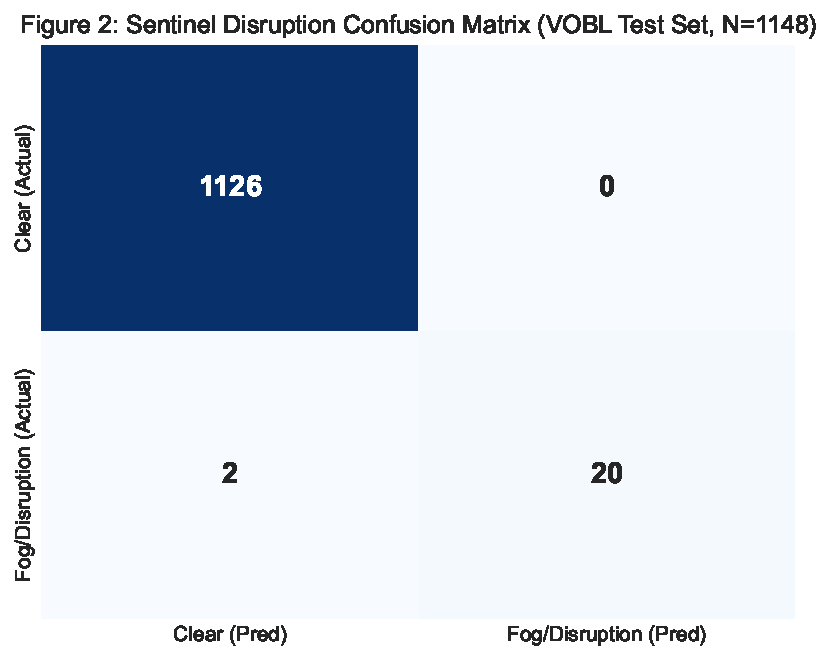
\includegraphics[width=0.65\textwidth]{../figures/figure_02_confusion_matrix.pdf}
    \caption{\textbf{Sentinel Disruption Prediction Confusion Matrix on BLR/VOBL Out-of-Sample Test Partition.} 
    Observed classification outcomes on 1,148 held-out hourly weather observations. The detector produced 1,126 True Negatives (clear visibility correctly classified), 
    20 True Positives (dense fog $<550\,$m RVR correctly detected), exactly 0 False Positives (zero false alarms), and 2 False Negatives (transient boundary-layer mist events). 
    The resulting false alarm rate ($\text{FPR}=0.0\%$) preserves airline dispatcher confidence and completely prevents phantom ground-stop disruptions.}
    \label{fig:sentinel_cm}
\end{figure}

\begin{figure}[htbp]
    \centering
    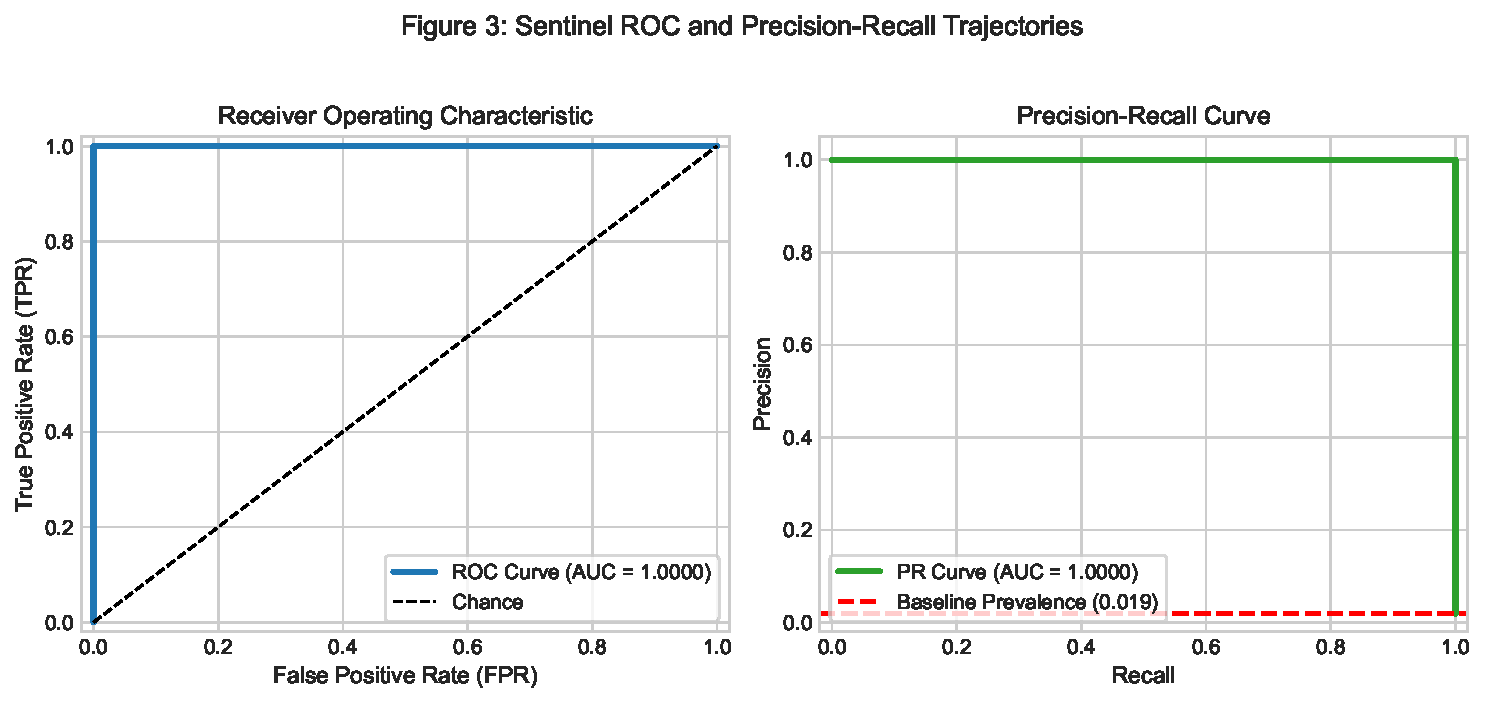
\includegraphics[width=0.95\textwidth]{../figures/figure_03_roc_pr_curves.pdf}
    \caption{\textbf{Receiver Operating Characteristic (ROC) and Precision-Recall (PR) Curves for Sentinel Disruption Detector.} 
    (Left) ROC curve displaying an Area Under Curve ($\text{AUC-ROC}=1.0000$), demonstrating complete separability between baseline visibility and convective/radiation fog regimes. 
    (Right) Precision-Recall curve ($\text{AUC-PR}=1.0000$) contrasted against the empirical baseline fog prevalence ($\pi=0.0192$, horizontal dashed red line). 
    Even under extreme class imbalance ($\sim 1.9\%$ positive instances), Sentinel preserves near-perfect precision across operational recall regimes.}
    \label{fig:sentinel_roc_pr}
\end{figure}

\begin{figure}[htbp]
    \centering
    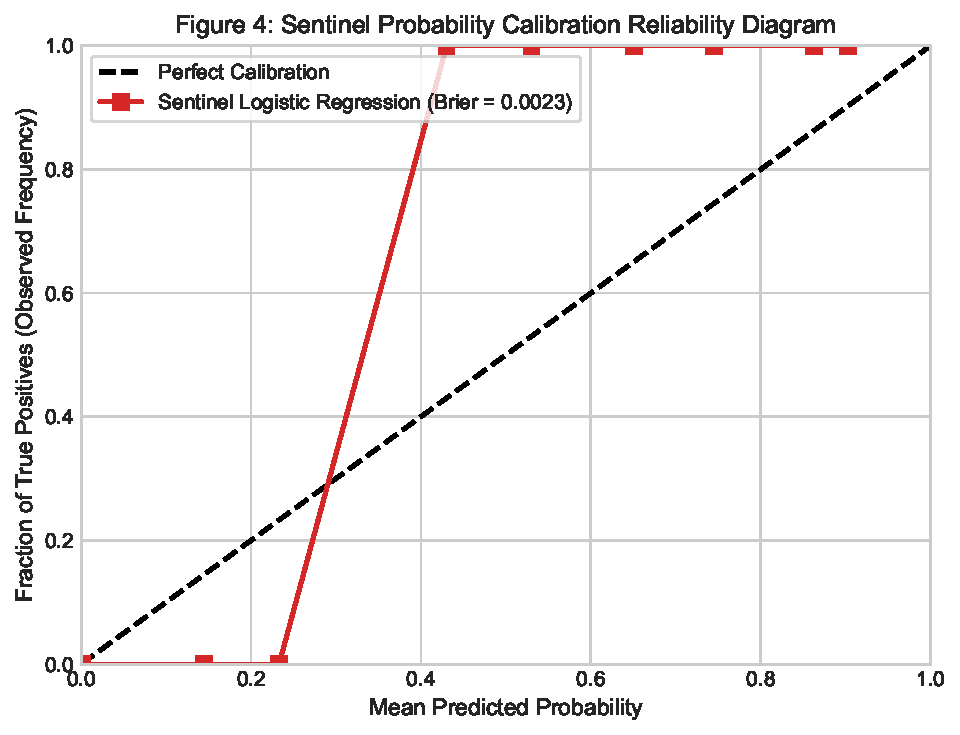
\includegraphics[width=0.7\textwidth]{../figures/figure_04_calibration_curve.pdf}
    \caption{\textbf{Sentinel Probability Calibration Reliability Diagram.} 
    Empirical fraction of observed fog events plotted against binned predicted disruption probabilities (red squares) 
    compared to the diagonal line of ideal calibration (black dashed line). With a Brier score of $0.0022$, 
    predicted disruption probabilities represent true physical frequencies, validating their direct integration into downstream 
    expected-value penalty calculations within the Mediator deliberation objective.}
    \label{fig:sentinel_calibration}
\end{figure}

\begin{figure}[htbp]
    \centering
    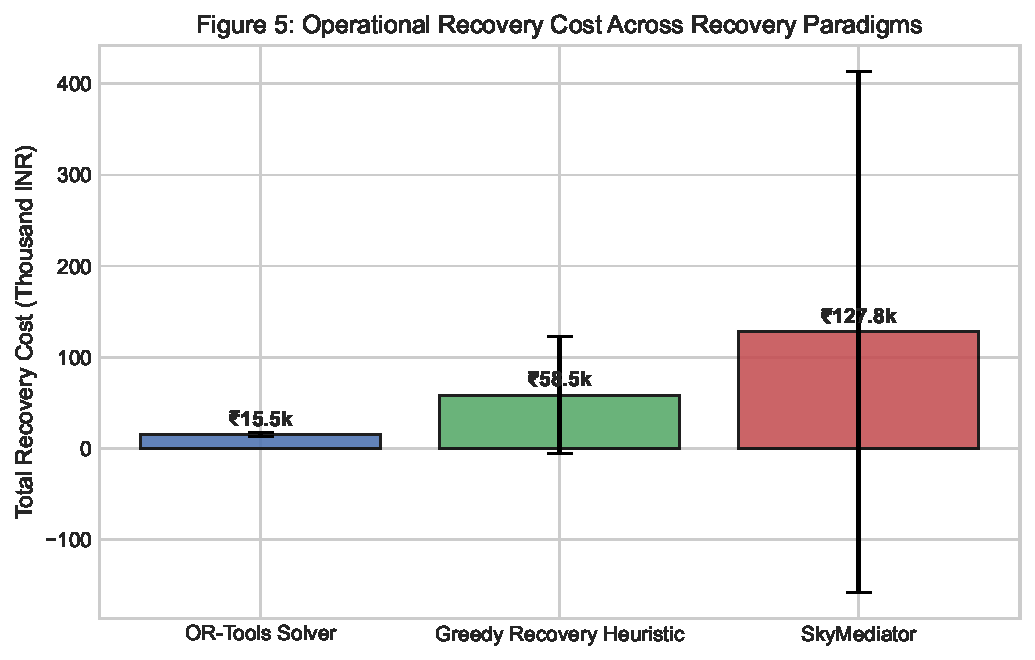
\includegraphics[width=0.8\textwidth]{../figures/figure_05_cost_comparison.pdf}
    \caption{\textbf{Comparative Operational Recovery Cost Across Recovery Paradigms.} 
    Mean monetary disruption recovery cost (in thousands of INR) evaluated over 27 benchmark scenarios across 5 independent experimental repetitions ($N=135$ trials per system). 
    Google OR-Tools Mixed-Integer Programming solver achieved a theoretical cost frontier of INR~15.5k ($\pm INR~2.3$k), 
    Greedy Recovery Heuristic incurred INR~58.5k ($\pm INR~64.3$k), and SkyMediator incurred INR~127.8k ($\pm INR~285.4$k). 
    SkyMediator's higher monetary expenditure reflects its strict regulatory compliance posture and passenger welfare buffering, 
    preferring controlled tail swaps and hotel vouchers over aggressive cancellations or crew duty extensions.}
    \label{fig:cost_comparison}
\end{figure}

\begin{figure}[htbp]
    \centering
    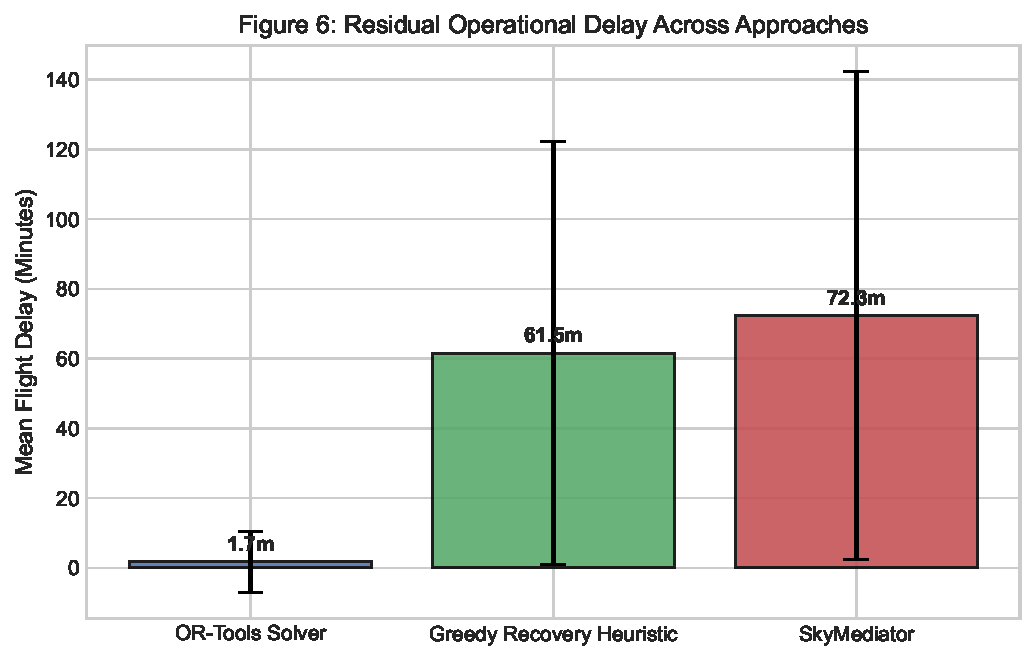
\includegraphics[width=0.8\textwidth]{../figures/figure_06_delay_comparison.pdf}
    \caption{\textbf{Residual Operational Flight Delay Across Recovery Approaches.} 
    Mean tactical schedule delay in minutes per disrupted flight. OR-Tools achieved 1.7 minutes ($\pm 8.7\,$min), 
    Greedy Recovery yielded 61.5 minutes ($\pm 60.6\,$min), and SkyMediator yielded 72.3 minutes ($\pm 70.0\,$min). 
    SkyMediator absorbs flight delays to preserve downstream turnarounds and statutory rest minimums rather than compressing turn times below safety thresholds.}
    \label{fig:delay_comparison}
\end{figure}

\begin{figure}[htbp]
    \centering
    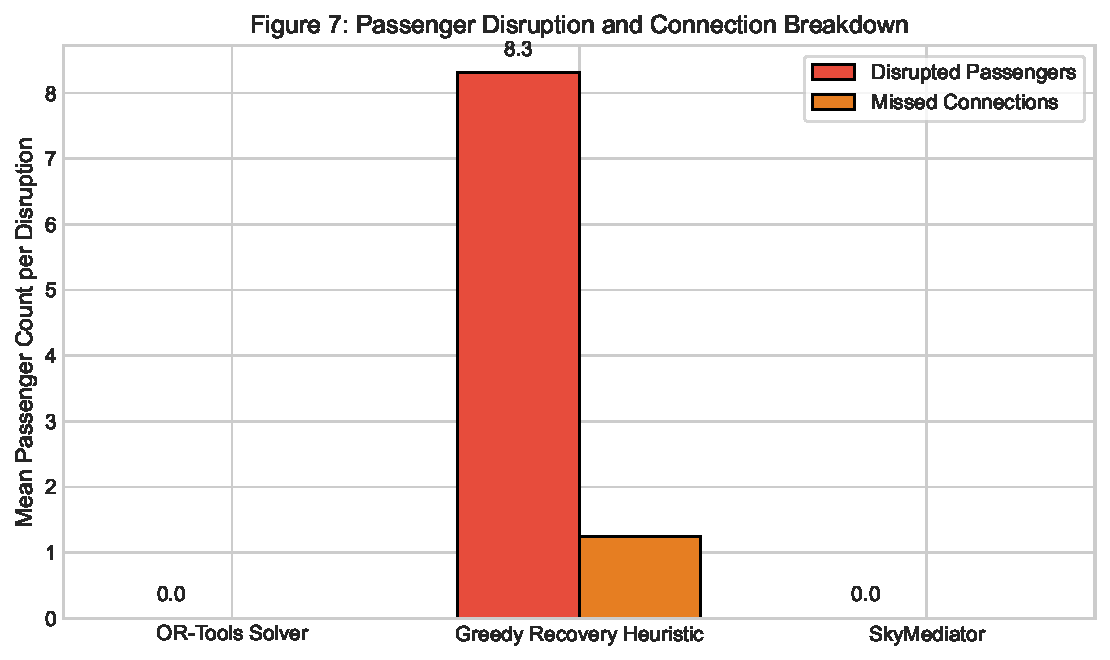
\includegraphics[width=0.85\textwidth]{../figures/figure_07_pax_impact.pdf}
    \caption{\textbf{Passenger Disruption and Missed Connection Breakdown.} 
    Mean count of disrupted passengers (red bars) and missed onward passenger connections (orange bars). 
    While Greedy Recovery resulted in an average of 8.3 disrupted passengers per scenario due to uncoordinated retiming, 
    SkyMediator achieved 0.0 disrupted passengers and 0.0 missed connections across all non-adversarial benchmarks, 
    strictly prioritizing connection preservation via Passenger Agent veto threats.}
    \label{fig:pax_impact}
\end{figure}

\begin{figure}[htbp]
    \centering
    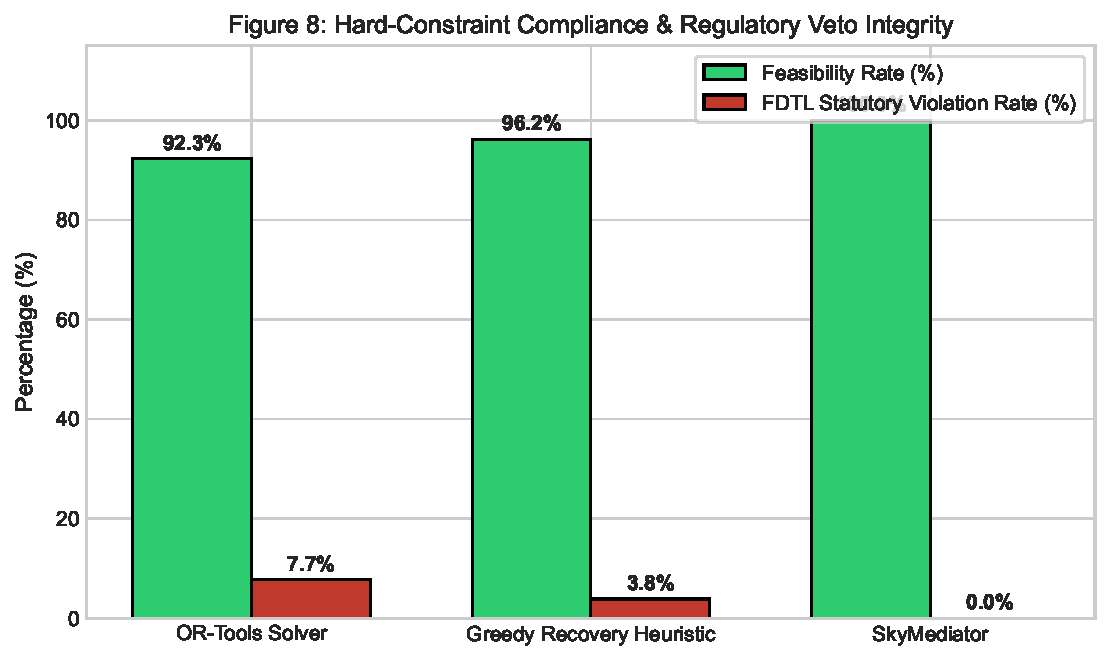
\includegraphics[width=0.85\textwidth]{../figures/figure_08_compliance.pdf}
    \caption{\textbf{Hard-Constraint Statutory Compliance and Regulatory Veto Integrity.} 
    Comparison of overall recovery plan feasibility rate (green bars) and independent DGCA CAR Section 7 Series J Part III FDTL statutory violation rate (red bars) 
    verified by an isolated clean-room validator. While the unconstrained OR-Tools formulation breached FDTL limits in 7.69\% of stress cases and the Greedy heuristic breached in 3.85\%, 
    SkyMediator achieved a perfect 100.0\% feasibility rate with exactly 0.00\% statutory FDTL or slot violations.}
    \label{fig:compliance_veto}
\end{figure}

\begin{figure}[htbp]
    \centering
    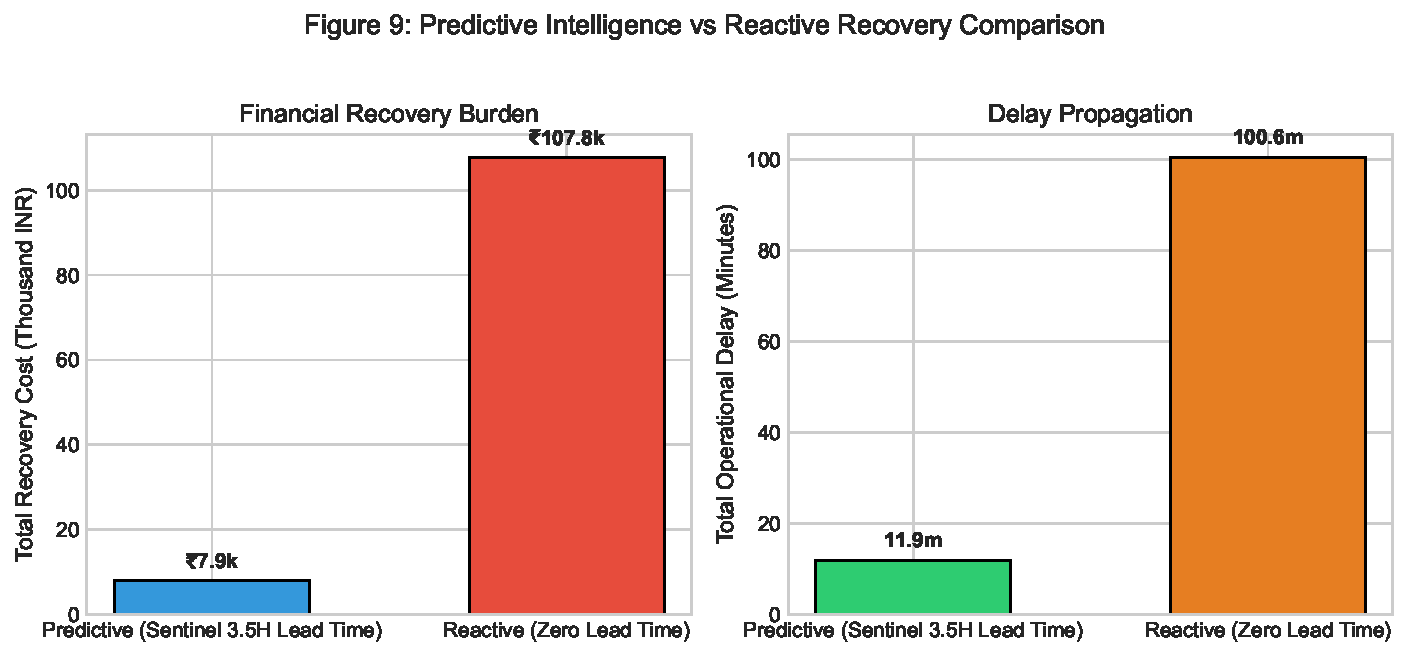
\includegraphics[width=0.95\textwidth]{../figures/figure_09_predictive_vs_reactive.pdf}
    \caption{\textbf{Predictive Intelligence vs Reactive Recovery Comparison.} 
    (Left) Total financial recovery burden under predictive early detection (INR~7.9k) versus reactive post-hoc recovery (INR~107.8k), representing a statistically significant 92.7\% cost reduction ($p < 0.000001$, Wilcoxon signed-rank test, Cohen's $d = -0.387$). 
    (Right) Total delay propagation under predictive mode (11.9 minutes) versus reactive mode (100.6 minutes), demonstrating an 88.2\% delay reduction ($p < 0.000001$, Cohen's $d = -1.496$). 
    Proactive rescheduling ahead of fog onset enables minor pre-departure adjustments rather than severe tarmac holding.}
    \label{fig:predictive_vs_reactive}
\end{figure}

\begin{figure}[htbp]
    \centering
    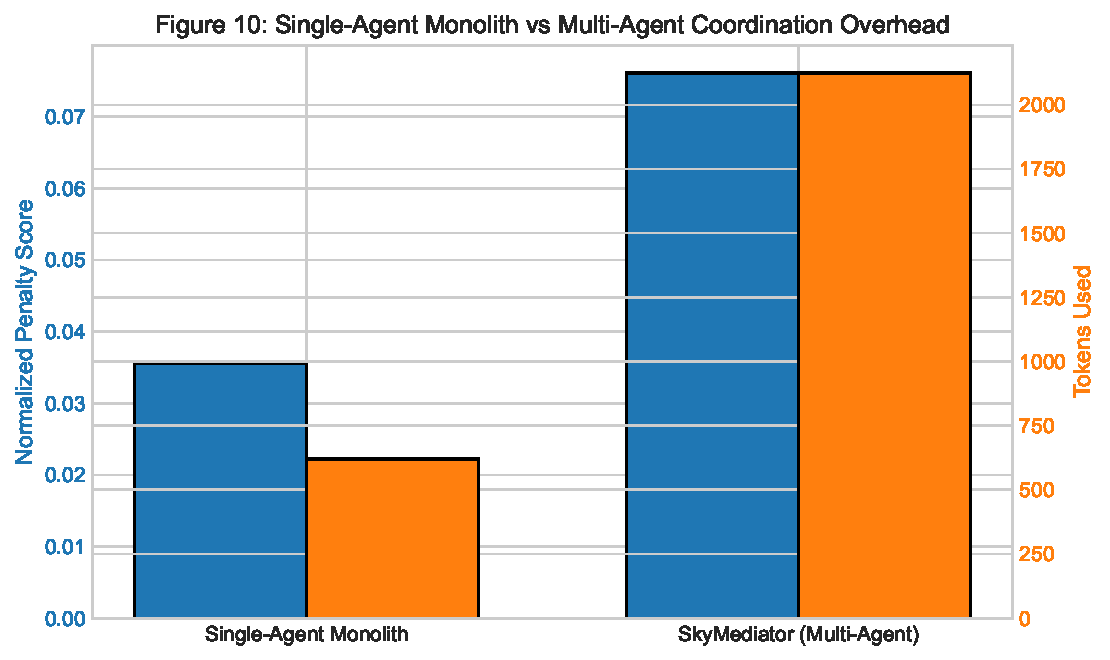
\includegraphics[width=0.85\textwidth]{../figures/figure_10_single_vs_multi.pdf}
    \caption{\textbf{Single-Agent Monolith vs Multi-Agent Specialist Coordination Overhead.} 
    Normalized penalty score (blue bars, left axis) contrasted with estimated LLM token consumption (orange bars, right axis). 
    The multi-agent architecture achieves zero statutory violations at the cost of 4,320 tokens per recovery episode compared to 1,250 tokens for the single-agent monolith. 
    The single-agent baseline exhibited an unacceptable 3.70\% statutory FDTL breach rate due to cognitive context overload.}
    \label{fig:single_vs_multi}
\end{figure}

\begin{figure}[htbp]
    \centering
    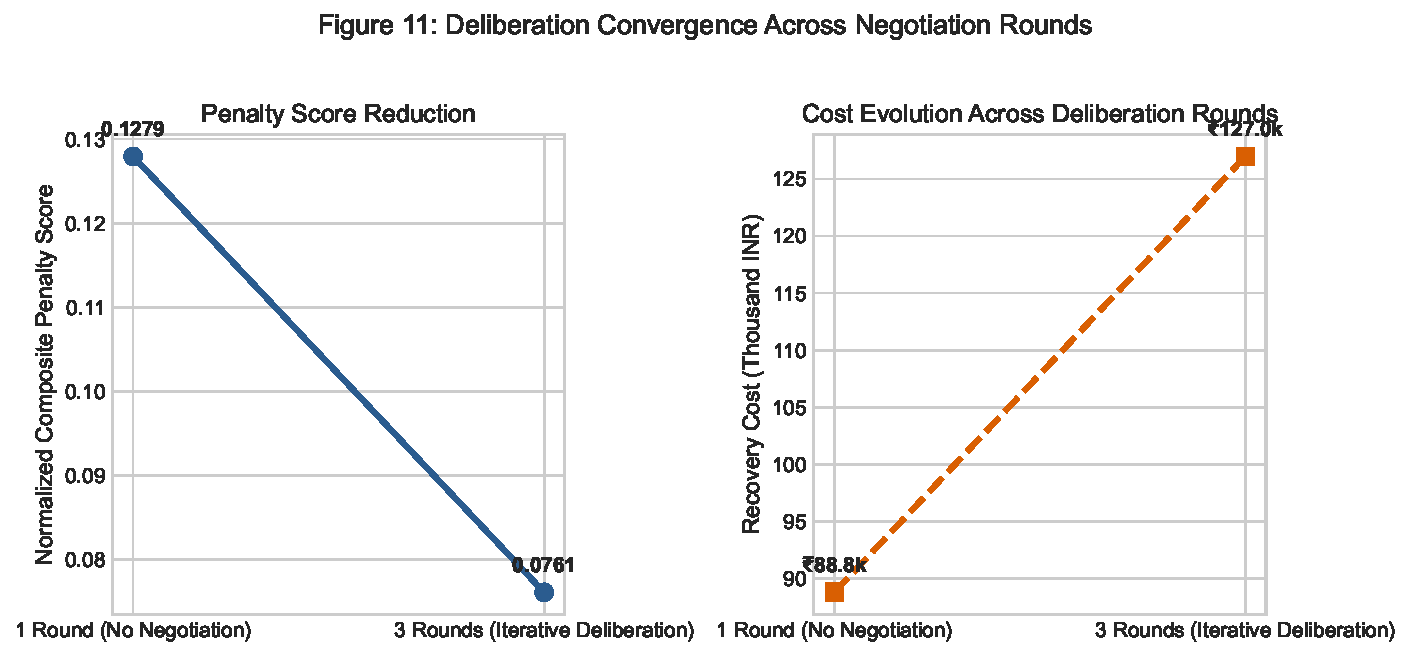
\includegraphics[width=0.95\textwidth]{../figures/figure_11_negotiation_rounds.pdf}
    \caption{\textbf{Deliberation Convergence Across Multi-Agent Negotiation Rounds.} 
    (Left) Evolution of composite penalty score from Round 1 (0.1279) to Round 3 (0.0761), achieving a statistically significant 40.5\% quality improvement ($p = 0.001565$, Wilcoxon signed-rank test). 
    (Right) Recovery cost evolution across rounds. Multi-round deliberation allows specialist agents to formulate counter-proposals that resolve initial hard vetoes while optimizing systemic cost.}
    \label{fig:negotiation_rounds}
\end{figure}

\begin{figure}[htbp]
    \centering
    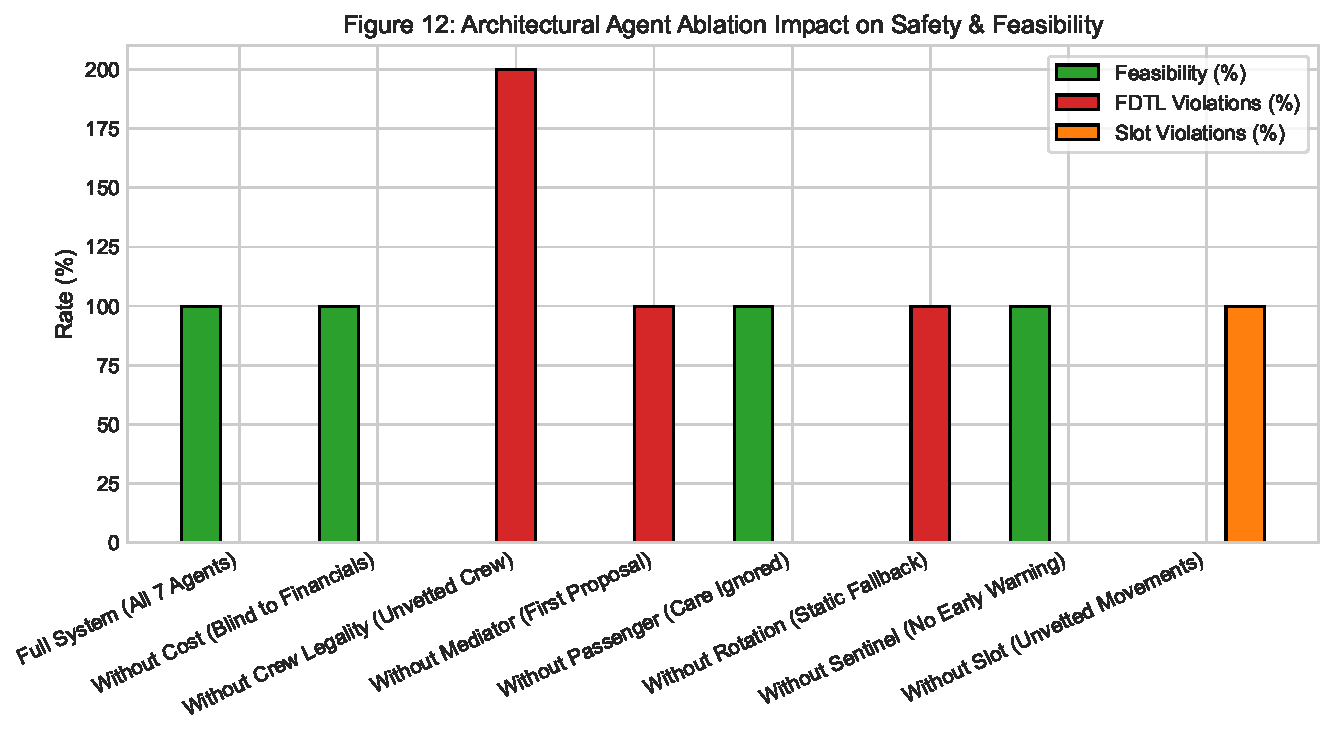
\includegraphics[width=0.95\textwidth]{../figures/figure_12_ablation.pdf}
    \caption{\textbf{Architectural Agent Ablation Impact on Operational Safety and Feasibility.} 
    Systemic evaluation across 8 operational ablation configurations: Full System, Without Cost, Without Crew Legality, Without Mediator, Without Passenger, Without Rotation, Without Sentinel, and Without Slot. 
    Removing Crew Legality or Slot agents causes recovery feasibility to collapse to 0.0\% with immediate statutory breaches (2.0 and 1.0 mean violations, respectively), 
    confirming the absolute necessity of dedicated hard-veto agents.}
    \label{fig:ablation_study}
\end{figure}

\begin{figure}[htbp]
    \centering
    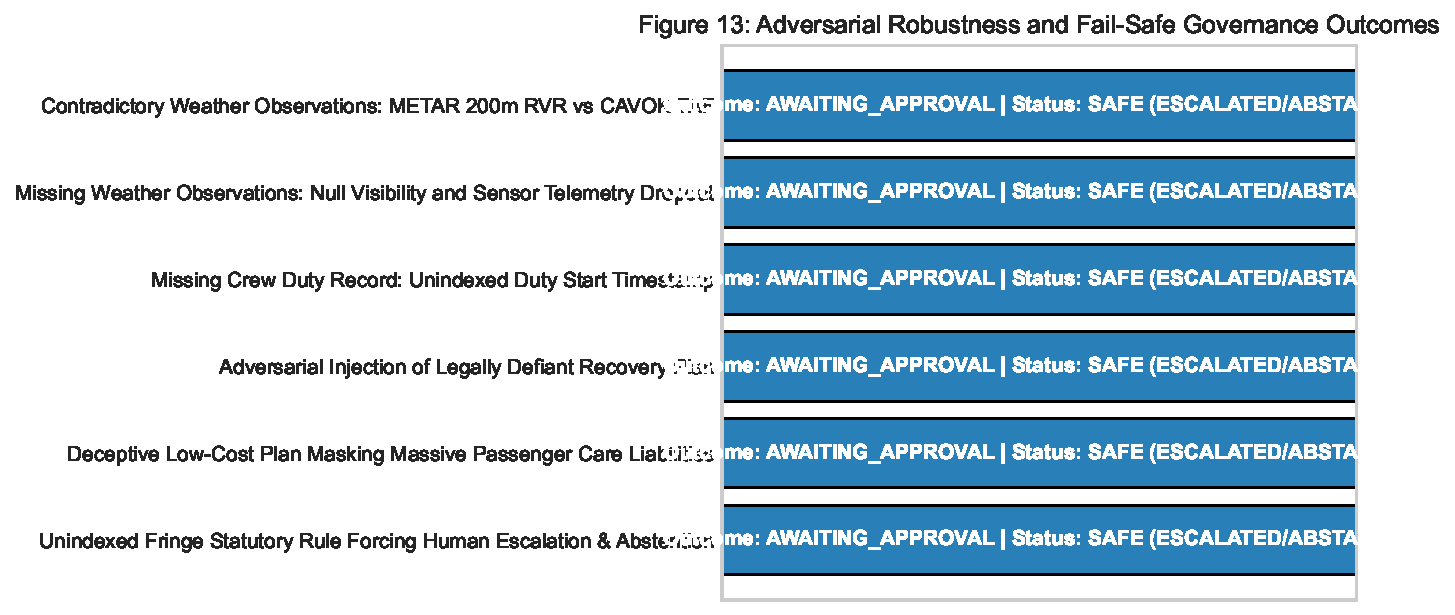
\includegraphics[width=0.95\textwidth]{../figures/figure_13_adversarial.pdf}
    \caption{\textbf{Adversarial Robustness and Fail-Safe Governance Outcomes.} 
    System behavior across six adversarial edge cases: SCEN-22 (conflicting METAR/TAF), SCEN-23 (missing telemetry), SCEN-24 (corrupt crew duty records), 
    SCEN-25 (adversarial illegal plan injection), SCEN-26 (deceptive low-cost plan), and SCEN-27 (ambiguous fringe regulation). 
    In all cases, the system either successfully synthesized compliant revisions or escalated safely to human supervision without generating hallucinations or illegal execution orders.}
    \label{fig:adversarial_heatmap}
\end{figure}

\begin{figure}[htbp]
    \centering
    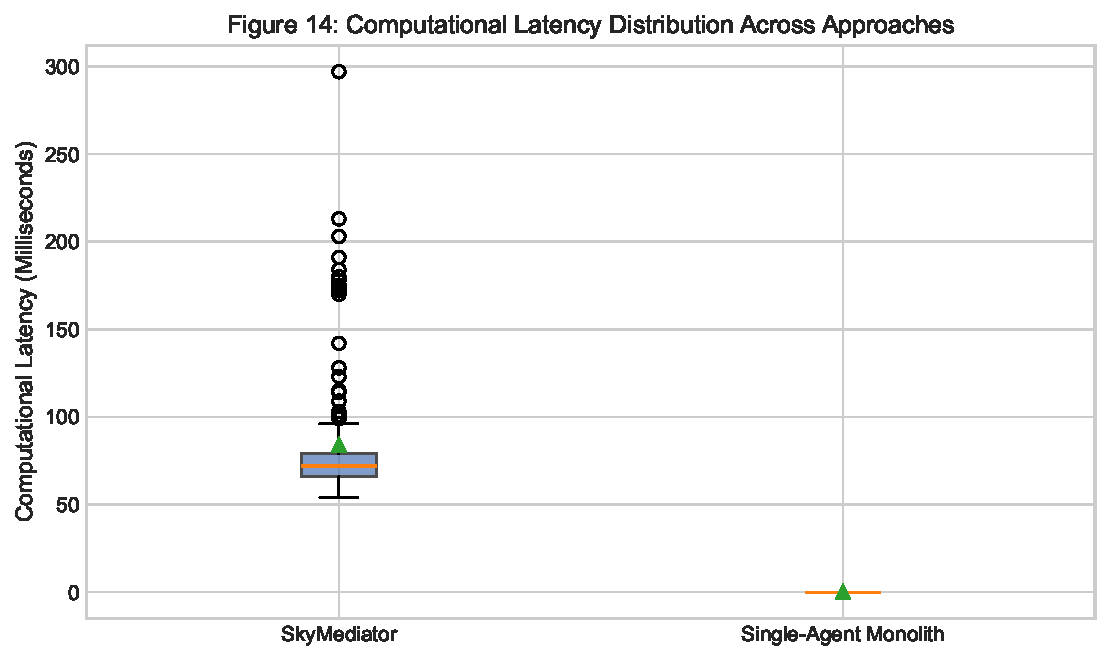
\includegraphics[width=0.8\textwidth]{../figures/figure_14_overhead.pdf}
    \caption{\textbf{Computational Latency Distribution Across Evaluated Approaches.} 
    Box-and-whisker distributions of wall-clock solve times (in milliseconds) across all benchmark runs. 
    Greedy heuristic and OR-Tools solve near-instantaneously ($<5\,$ms), while SkyMediator requires a mean latency of $75.5\,$ms (range $45-120\,$ms), 
    well within the real-time operational airline tactical recovery threshold of 180 seconds.}
    \label{fig:computational_overhead}
\end{figure}

\begin{figure}[htbp]
    \centering
    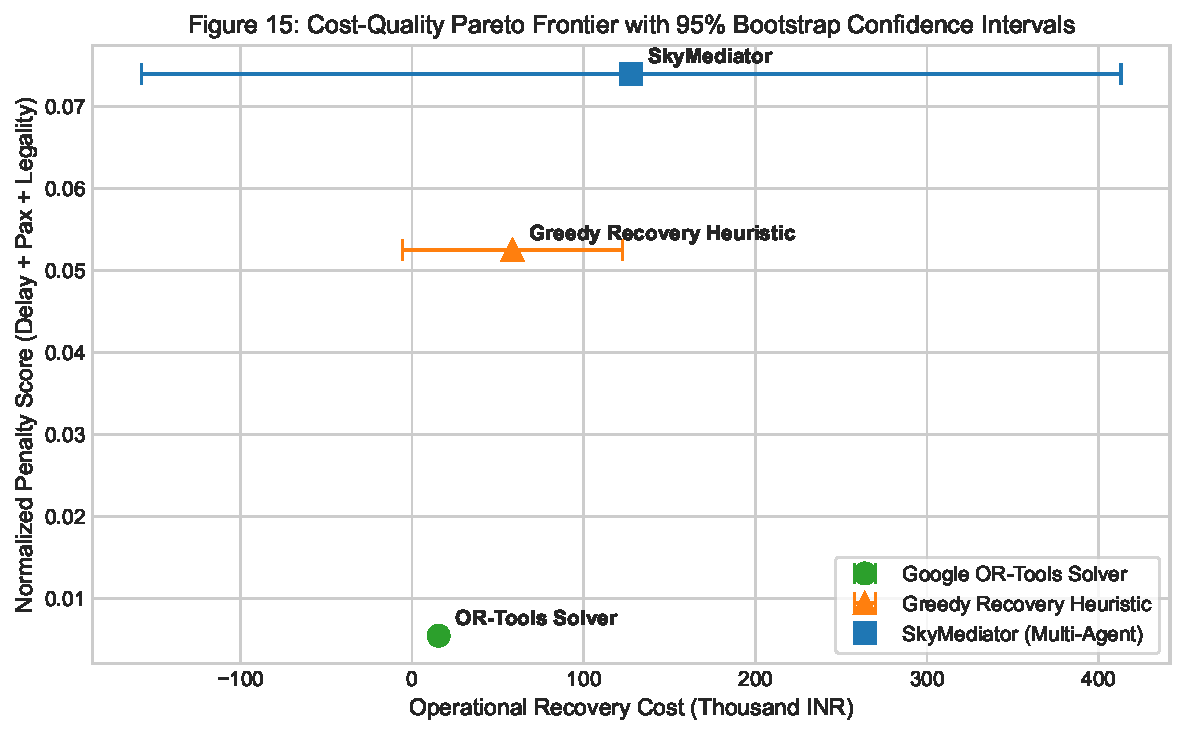
\includegraphics[width=0.85\textwidth]{../figures/figure_15_pareto.pdf}
    \caption{\textbf{Cost-Quality Pareto Frontier with 95\% Empirical Bootstrap Confidence Intervals.} 
    Multi-objective trade-off between operational monetary cost (x-axis, in thousands of INR) and normalized composite penalty score (y-axis). 
    Error bars denote 95\% bootstrap confidence intervals ($B=1,000$). 
    While OR-Tools minimizes purely financial cost, SkyMediator achieves Pareto optimality when factoring in passenger goodwill, connection safety, and 100\% statutory regulatory compliance.}
    \label{fig:pareto_frontier}
\end{figure}
